\chapter{Engineering model}
This chapter will describe engineering model developed during this thesis.

This model should be as close to flight model as possible - but it could be e.g. on separate board, which is this case.

This model was developed as flight-ready version for sensor calibration \& tests along with developing \& testing flight software.

\section{Background - calibration stand}
    During development of the system previous model was developed to test and calibrate MOSFET transistors to use as a radiation dosimeters. Calibration stand was developed by M. Gumiela in his engineering thesis \cite{MGThesis}. The basic goal was to develop measurement device which can be used to determine final operational point, calibrate radiation response and to perform temperature calibration of flight sensor.

    TODO: opis stanowiska


\section{Block diagram}
    Block diagram of proposed system based on CD4007 is presented on figure TODO.

    It was designed having in mind miniaturization of sensor - to fit on PW-Sat2 PLD board. Because CD4007 has 3 complementary MOS pairs it was proposed to use all of them - to improve fidelity of the measurements. One n-MOS is used as a temperature sensor.

    Current source and ADC are multiplexed between 4 channels - 3x p-MOS and 1x n-MOS. This reduces board space and sensor accuracy (1 current source/ADC can be more sophisticated).

\section{Low-level requirements}
    Using design requirements \ref{Design_requirements} and characteristic curves from \ref{Characteristic_curves} low-level specifications were assumed:
    \begin{itemize}
        \item operating temperature range: $0 \div 60 \si{\degreeCelsius}$,
        \item current source value: $\SI{100}{\micro\ampere} \pm \SI{10}{\nano\ampere}$,
        \item ADC resolution: $TODO$,
        \item ADC accuracy: $TODO$,
        \item Noise floor on ADC: $TODO$
    \end{itemize}


\section{Analog front-end}
    In this section decision and schematic diagrams of building blocks are presented.

    \subsection{SPICE models}
        Design should be validated by simulation. To make this possible, model of every device should be accessible.

        For CD4007 model RIT4007P7 from Rochester Institute of Technology \cite{RIT_FULLER} was used.

    \subsection{Linear regulator}
        Important part of design - power supply for analog circuitry. Because $+\SI{5}{V}$ rail from EPS is an output from DC-DC converter (which runs on \SI{500}{\kilo\hertz}) the analog supply voltage have to be very well regulated and filtered. Because line from satellite bus is \SI{5}{\volt} and to run current source there is a need for as high voltage as possible LDO output voltage was selected to be \SI{4.5}{\volt}.

        As an Low Dropout Voltage LT3042 was selected. It is ultralow Noise, ultrahigh PSRR RF linear regulator by Linear Technology. Key specs:
        \begin{itemize}
            \item ultralow noise \SI{0.8}{\micro\volt RMS} (\SI{10}{\hertz} to \SI{100}{\kilo\hertz}),
            \item output current \SI{200}{\milli\ampere}
            \item input range \SI{1.8}{\volt} to \SI{20}{\volt}, output range \SI{0}{\volt} to \SI{15}{\volt}
            \item ultrahigh PSRR \SI{79}{\decibel} at \SI{500}{\kilo\hertz}
        \end{itemize}

    \subsection{Current source}
        Current source have to be the most accurate part of the design, because measured voltage depends in square of its variation. It was assumed that $\SI{50}{\nano\ampere}$ current stability across temperature and aging range will be sufficient.

        Main concept of current source is based on Burr-Brown application note \cite{Make_a_precision_current_source_or_sink}. Idea schematic is shown on figure \ref{current_source_schematic}.

        \begin{figure}[H]
            \centering
            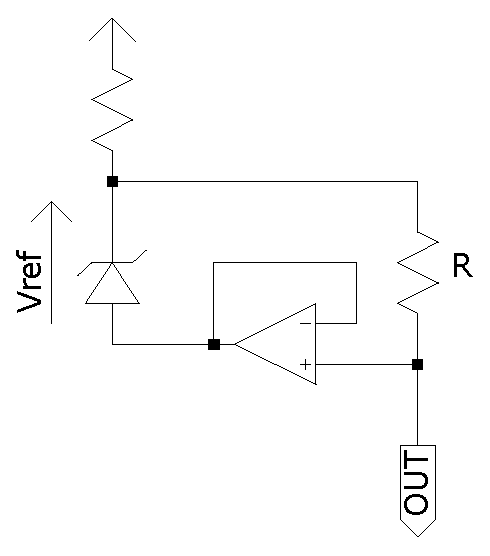
\includegraphics[width=0.3\paperwidth]{img/06/current_source_schematic.eps}
            \caption{Threshold voltage readout block diagram}
            \label{current_source_schematic}
        \end{figure}

        Output current is set by shunt voltage reference and resistor $R$, it is given by equation:
        $$I_{OUT} = V_{ref}/R$$

        Therefore, stability of output current depends on reference voltage and resistor accuracy.

        \bigskip \textbf{Shunt reference}

        After irradiation MOSFET $V_{DS}$ is planned to be about \SI{2.5}{\volt}, so reference voltage have to have voltage less than \SI{2}{\volt}.

        Linear Technology LT1634-1.25 shunt voltage reference was chosen. It is one of the best shunt references from LT. Basic specification:
        \begin{itemize}
            \item \SI{0.05}{\percent} initial accuracy,
            \item \SI{10}{ppm/\degreeCelsius} maximum temperature drift,
            \item $< \SI{1}{\ohm}$ dynamic resistance
        \end{itemize}

        Shunt resistance was chosen to make a current flowing through reference about $10-\SI{20}{\micro\ampere}$ - value of \SI{5}{\kilo\ohm}.

        \bigskip \textbf{Series resistor}

        Value of this resistor reflects required current flowing through MOSFET. Nominal value selected was $TODO$.

        Critical in this resistor is stability across temperature, it directly reflects changes in current. For achieving requirements \SI{10}{\kilo\ohm} / \SI{5}{ppm} was chosen (APC0603T10K0Z).

        Manufacturer does not specify profile of the temperature coefficient - so both worst cases was simulated (\SI{-5}{ppm} and \SI{5}{ppm}).

        \bigskip \textbf{Operational amplifier}

        Operational amplifier in this circuit have very low bandwidth (noise limitation), low offset voltage (precision) and small footprint. LTC2054 was selected - key characteristics:
        \begin{itemize}
            \item \SI{3}{\micro\volt} offset voltage,
            \item common mode $\pm \SI{0.5}{\volt}$ input/output range,
            \item \SI{500}{\kilo\hertz} gain-bandwidth product,
            \item device in Military Plastic package (temperature range $-55 \div \SI{150}{\degreeCelsius}$)
        \end{itemize}

        \bigskip \textbf{Simulation}

        Full behavioral simulation was performed in LTSpice. MOSFET was replaced by resistance emulating its static resistance ($\SI{2}{\volt}/\SI{125}{\micro\ampere} = \SI{16}{\kilo\ohm}$). Simulation view is shown on figure \ref{current_source_simulation}.

        \begin{figure}[H]
            \centering
            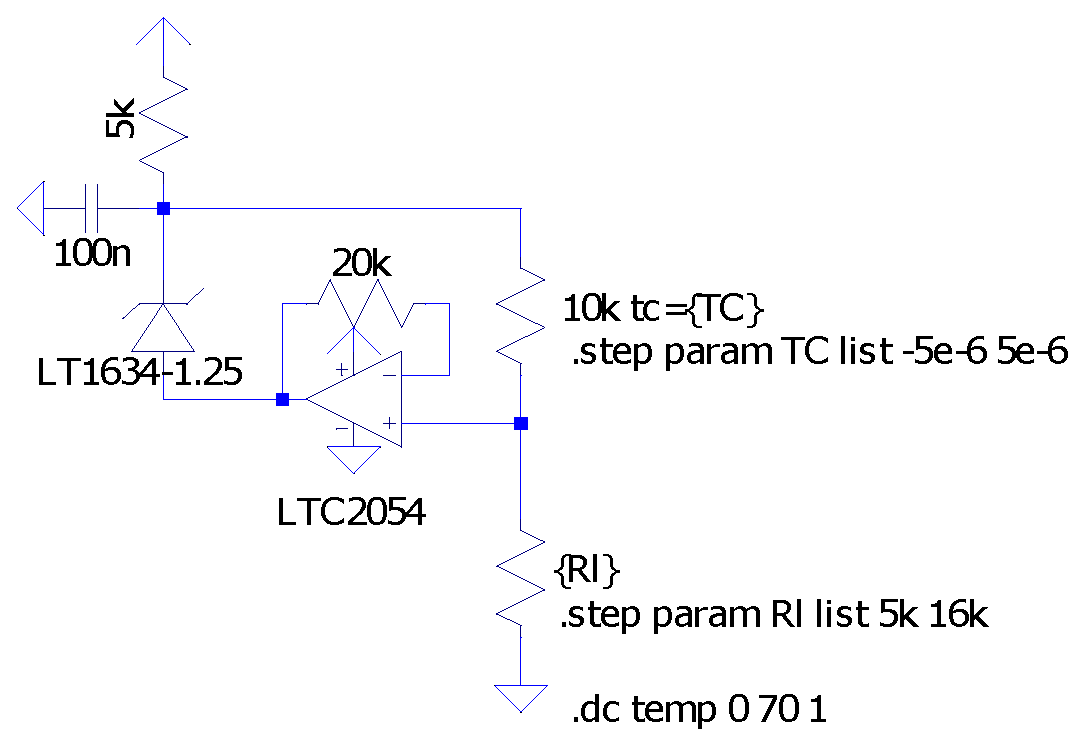
\includegraphics[width=0.5\paperwidth]{img/06/current_source.eps}
            \caption{Current source simulation}
            \label{current_source_simulation}
        \end{figure}

        Result (output current):

        \begin{figure}[H]
            \centering
            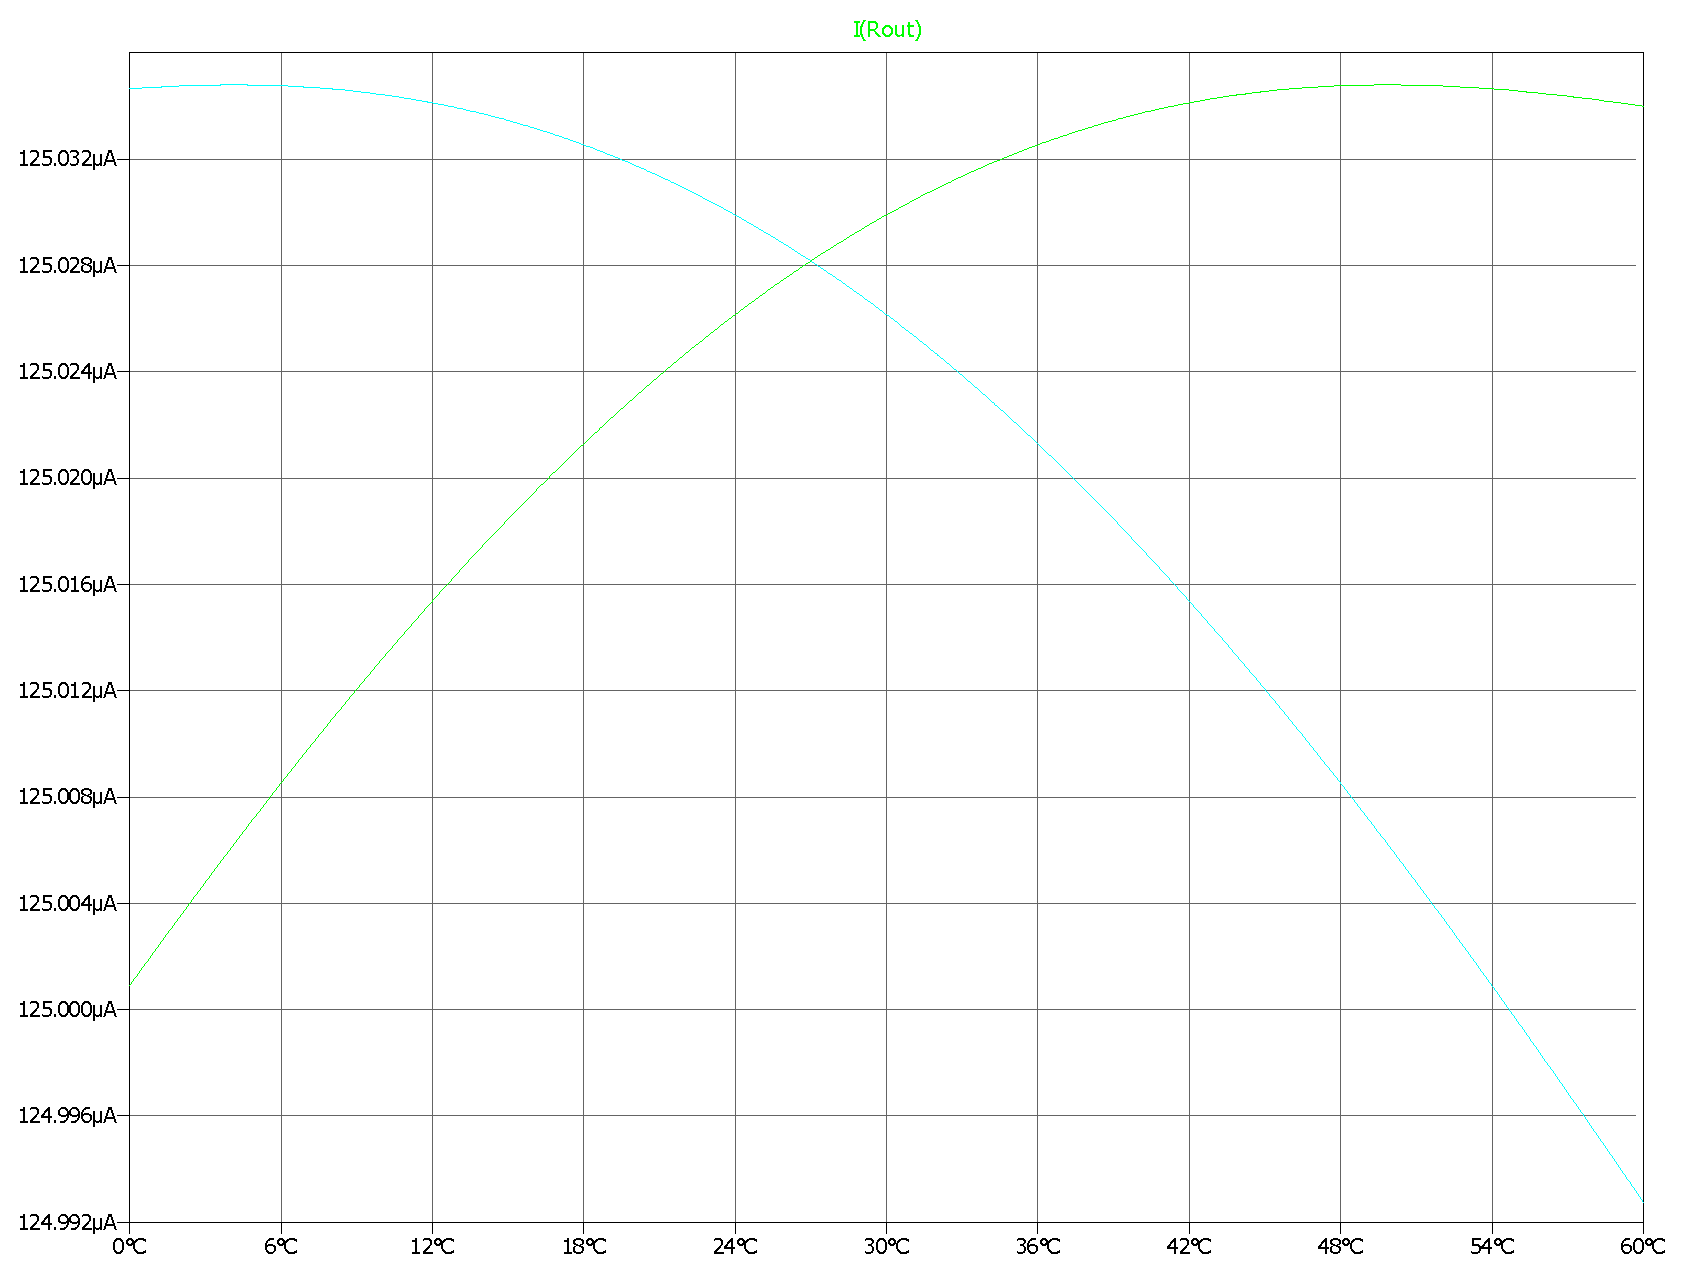
\includegraphics[width=0.8\paperwidth]{img/06/current_source_result.eps}
            \caption{Current source simulation result - output current}
            \label{current_source_simulation_result}
        \end{figure}

        In both cases current change across temperature range does not exceed \SI{40}{\nano\ampere}.

    \subsection{ADC}
        Analog to digital converter is responsible for reading $V_{DS}$ voltage across transistor. Due to very low changes high accuracy and resolution is required. Additionally, complex digital element like ADC should have radiation tests to prove its reliability. To achieve at least \SI{0.1}{\milli\volt} resolution ADC has to be at least \SI{16}{bits}.

        Due to constrain on system and reliability the AD7714 from Analog Devices was chosen. Radiation tests for this device can be found at TODO. Internal diagram can be found on figure \ref{AD7714}. Key specs:
        \begin{itemize}
            \item \SI{24}{bits},
            \item \SI{0.0015}{\percent} nonlinearity,
            \item programmable gain ($1 \div 128$),
            \item 3 fully differential or 5 pseudo-differential input channels
            \item \SI{3}{\volt} or \SI{5}{\volt} operation
            \item separated digital and analog supply and grounds,
            \item SPI interface
        \end{itemize}

        \begin{figure}[H]
            \centering
            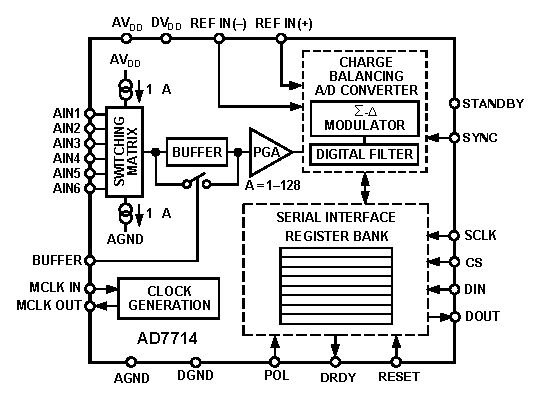
\includegraphics[width=0.5\paperwidth]{img/06/AD7714.eps}
            \caption{AD7714 internal block diagram. Source: TODO}
            \label{AD7714}
        \end{figure}

        This ADC is much too complex for this particular need, but it is the only one (apart from ADC128, but this is 12-bit) with radiation tests.

        AD7714 requires external crystal or clock oscillator in frequency range \SI{1}{\mega\hertz} to \SI{2.54}{\mega\hertz}. Crystal oscillators for these frequencies are large and susceptible for shocks and damages because of large, delicate internal structure (firure \ref{Opening_a_Quartz_Crystal_Can_Effects_Thereof}). \SI{1}{\mega\hertz} ceramic oscillator ISM95-3351AH was selected for operation (figure \ref{ISM95-3351AH-1.0000}).

        \begin{figure}[H]
            \centering
            \includegraphics[width=0.5\paperwidth]{img/06/crystal.png}
            \caption{Low frequency crystal oscillator internals. Source: \cite{        Opening_a_Quartz_Crystal_Can_Effects_Thereof}}
            \label{Opening_a_Quartz_Crystal_Can_Effects_Thereof}
        \end{figure}

        \begin{figure}[H]
            \centering
            \includegraphics[width=0.5\paperwidth]{img/06/ISM95.png}
            \caption{ISM95-3351AH-1.0000 ceramic oscillator package. Source: TODO}
            \label{ISM95-3351AH-1.0000}
        \end{figure}


    \subsection{Multiplexer}
        Because CD4007 have three p-MOS transistors it was planned to read every channel. Space constrains does not allow to have four current sources (for p-MOS and n-MOS), therefore current have to be multiplexed. Additionally, ADC have only three differential input, so it was proposed to multiplex it as well.

        As an analog multiplexer ADG709 was chosen. Its radiation tests can be found in TODO. It is double 1:4 mux, allowing simultaneous current and voltage multiplexing. Internal block diagram is shown on figure \ref{ADG709_block}

        \begin{figure}[H]
            \centering
            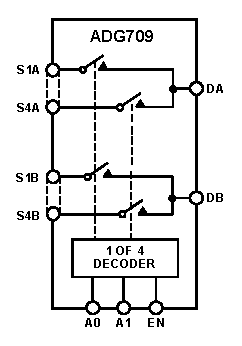
\includegraphics[width=0.3\paperwidth]{img/06/ADG709.eps}
            \caption{ADG709 internal block diagram. Source: TODO}
            \label{ADG709_block}
        \end{figure}

    \subsection{Differential filter}
        Internal sampling frequency of ADC (for GAIN = 1 and $f_{clk} = \SI{1}{\mega\hertz})$ is about \SI{15.6}{\kilo\hertz}. To eliminate aliasing and reduce readout noise low-pass differential filter should be implemented on ADC input.

        Simple one-pole RC filter was selected. Its schematic can be found on figure \ref{low_pass_filter}.

        \begin{figure}[H]
            \centering
            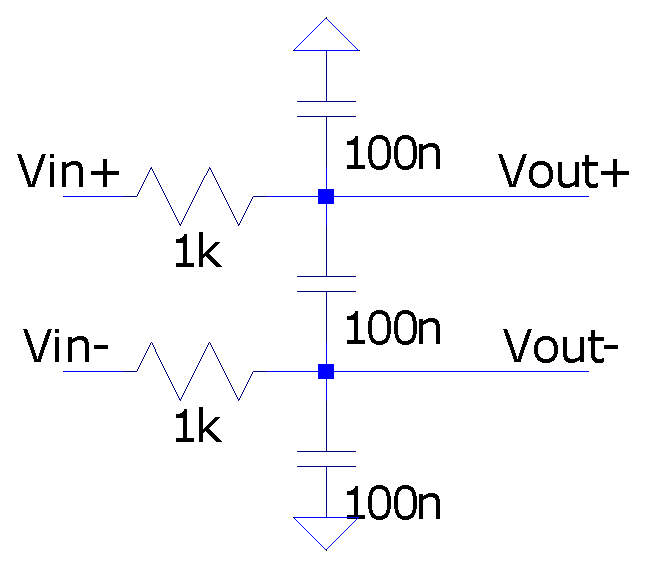
\includegraphics[width=0.3\paperwidth]{img/06/low_pass_filter.eps}
            \caption{Low pass filter schematic.}
            \label{low_pass_filter}
        \end{figure}

        Using AC analysis its frequency characteristic was obtained - figure \ref{low_pass_filter_output}. At half of sampling frequency attenuation is about \SI{22}{\decibel}.

        \begin{figure}[H]
            \centering
            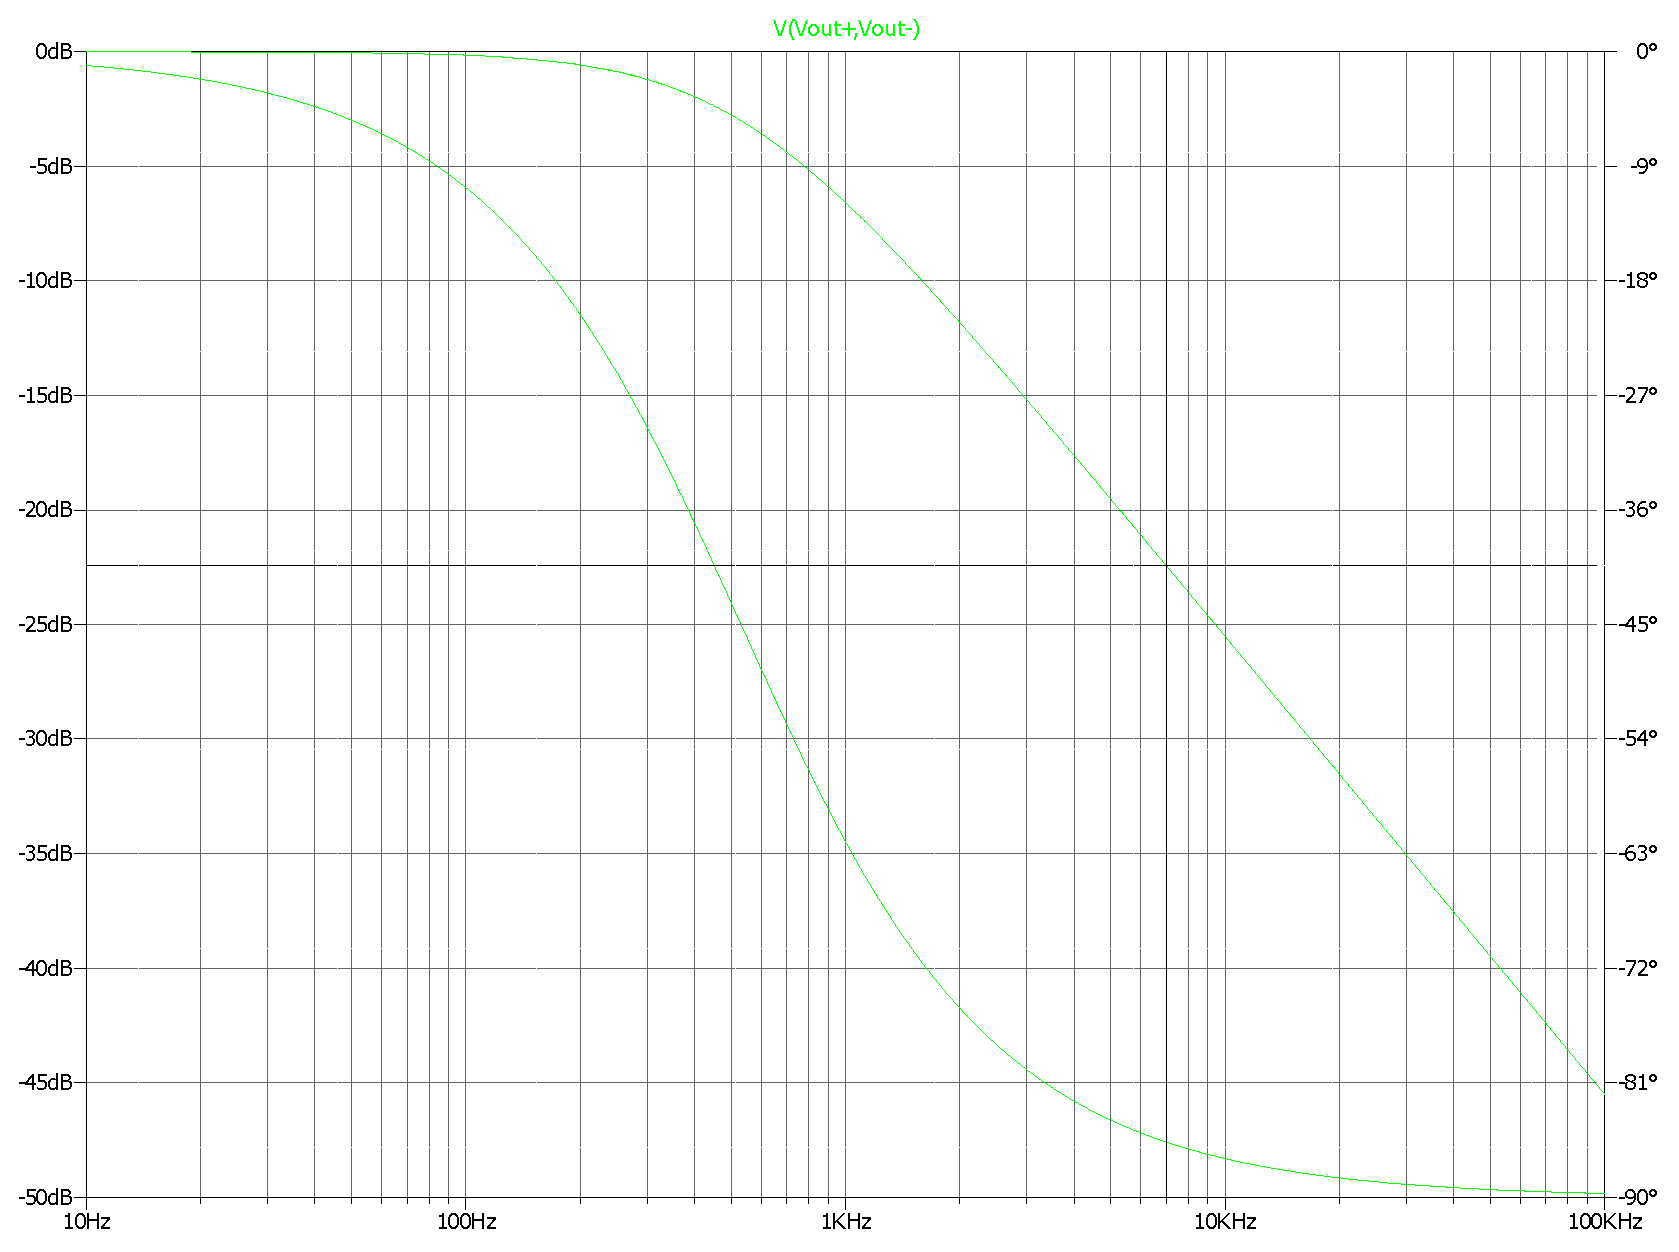
\includegraphics[width=0.7\paperwidth]{img/06/low_pass_filter_output.eps}
            \caption{Low pass filter frequency characteristics.}
            \label{low_pass_filter_output}
        \end{figure}

    \subsection{Shielding}
        Because of noise requirements and near proximity of \SI{0.5}{\watt} radio transmitter, EMI shielding was tested.

        Proper pads for EMI shielding were placed on PCB. Its size depends on PCB layout, after routing it was decided to use BMI-S-203 shield (figure \ref{BMI-S-203}). This shield should provide attenuation of about \SI{50}{\decibel} on transmitter frequency.

        \begin{figure}[H]
            \centering
            
\includegraphics[width=0.7\paperwidth]{img/06/BMI-S-203.eps}
            \caption{BMI-S-203 shield. Source: TODO}
            \label{BMI-S-203}
        \end{figure}


\section{Digital}
    RadFET is mainly analog sensor. But, ADC, MUX and LDO has to be controlled from on-board microcontroller. On other hand, RadFET have to be accessible from OBC, to retrieve data and send them to ground.

    \subsection{Microcontroller}
        Main digital part of the design is microcontroller. It will be responsible for:
        \begin{itemize}
            \item controlling analog part of the sensor,
            \item calculating values and implement FDIR for incorrect values,
            \item communicating with OBC to send data and transfer them to ground station for further analysis.
        \end{itemize}

        Couple of options were considered, and the final choose was ATmega164PV-10AQ.

        AVR devices are known from their simplicity, reliability and very little bugs. In addition, radiation tests were performed for ATmega series (TODO).

        Features of this particular device:
        \begin{itemize}
            \item \SI{1.8}{\volt} - \SI{5.5}{\volt} supply voltage,
            \item \SI{4}{\mega\hertz} clock,
            \item TQFP-44 package,
            \item \SI{16}{\kilo B} program memory,
            \item \SI{1}{\kilo B} SRAM
        \end{itemize}

    \subsection{OBC interface}
        Interface to OBC is $I^2C$ bus. Because sensor can be turned off by cutting its voltage proper buffering had to be implemented. For this purpose $I^2C$ repeater PCA9517 was placed in the design. Its functional diagram can be seen on figure \ref{PCA9517}. From its datasheet: "The SDA and SCL pins are over voltage tolerant and are high-impedance when the PCA9517 is unpowered." (TODO). Thanks to it OBC can completely disable the sensor, by simply cutting it a power.

        \begin{figure}[H]
            \centering
            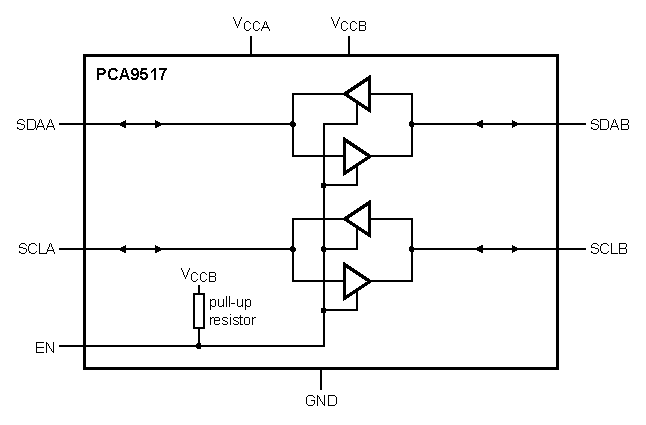
\includegraphics[width=0.7\paperwidth]{img/06/PCA9517.eps}
            \caption{PCA9517 internal block diagram. Source: TODO}
            \label{PCA9517}
        \end{figure}


\section{Final schematic}
    Top level schematic file can be seen on figure \ref{top_level_schematic}. Ports represents physical connectors - to satellite bus and debug socket.

    \begin{figure}[H]
        \centering
        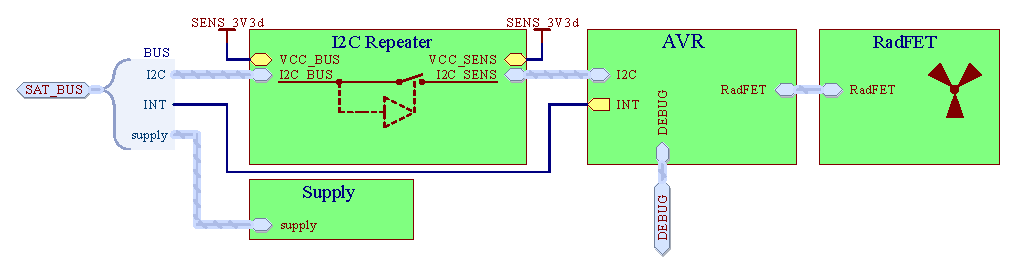
\includegraphics[width=0.8\paperwidth]{img/06/final_schematic_top.eps}
        \caption{Top level schematic}
        \label{top_level_schematic}
    \end{figure}

    "RadFET" consists analog part of the design. Its block diagram can be seen on figure \ref{analog_schematic}.

    \begin{figure}[H]
        \centering
        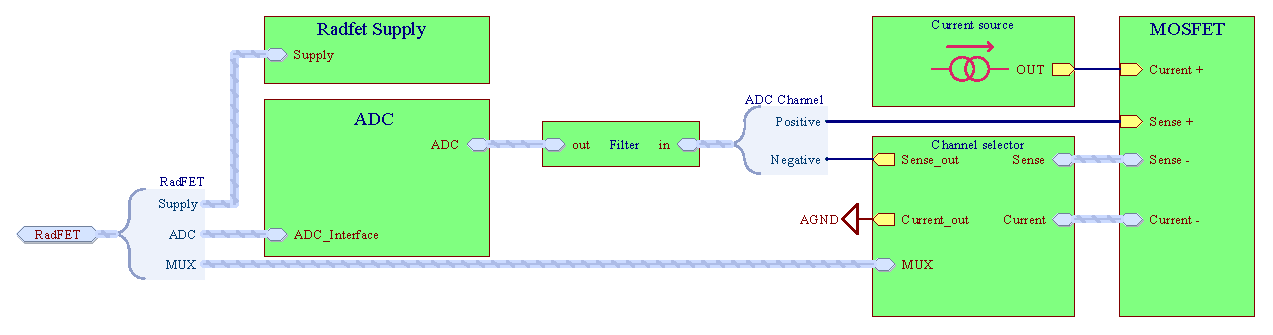
\includegraphics[width=0.8\paperwidth]{img/06/final_schematic_radfet.eps}
        \caption{Sensor final schematic - analog part}
        \label{analog_schematic}
    \end{figure}


\section{Software design}
    \subsection{AVR-HAL}
    \subsection{I2C-slave module}
    \subsection{Measurement algorithm}

\section{PCB}
    \subsection{PCB stack}
    \subsection{PCB layout}
    \subsection{3D model}
    \subsection{Manufacturing}

\section{Assembly}

\section{Finished sensor}
